\documentclass[11pt]{article} % For LaTeX2e
\usepackage{manuscript, palatino}
\usepackage{graphicx}
\usepackage{amsfonts, amsmath}
\usepackage{algorithm, algpseudocode}%

\usepackage{natbib}

\title{Title Pending}

\author{
Samuel Zorowitz \\
Princeton Neuroscience Institute\\
Princeton University\\
Princeton, NJ 08540 \\
\texttt{zorowitz@princeton.edu} \\
\And
Ida Momennejad \\
Columbia University\\
New York, NY 10027 \\
\texttt{ida.m@columbia.edu} \\
\And
Nathaniel Daw \\
Princeton Neuroscience Institute\\
Princeton University\\
Princeton, NJ 08540 \\
\texttt{ndaw@princeton.edu} \\
}

\newcommand{\fix}{\marginpar{FIX}}
\newcommand{\new}{\marginpar{NEW}}

\begin{document}

\maketitle

\begin{abstract}
Pending
\end{abstract}

\keywords{
decision theory; computational psychiatry; anxiety; value iteration
}

\startmain

\section{Introduction}

Many psychiatric disorders involve distortions to representations of the external world and, as a likely consequence, pronounced changes to learning and decision making. As a normative framework, decision theory allows us to describe and pose quantita­tive questions about optimal choice behavior \citep{DayanDaw2008} and is, therefore, a critical tool for modeling, understanding, and predicting the psychological and neurobiological mechanisms underlying psychiatric behavior \citep{maia2011, HuysDawDayan2015}. Recent investigations employing this framework have provided novel and important insights into psychiatric symptoms and disorders, including anhedonia in major depression \citep{Rutledge2017}, mood instability in bipolar disorder \citep{EldarNiv2015, EldarDolanNiv2016}, habitual behavior in obsessive compulsive and addictive disorders \citep{gillan2016}, and hallucinations in schizophrenia \citep{powers2017, corlett2018}.

The family of anxiety disorders (which includes generalized anxiety disorder, social anxiety disorder, panic disorder, and specific phobia) are characterized by excessive fear and worry about future negative outcomes, and represent the most common group of psychiatric disorders \citep{kessler2009}. Though the disorders typically differ in the types of objects or situations that induce fear or anxiety, all share a set of core disturbances to cognition and behavior. First, the anxiety disorders involve pessimistic inference, or a tendency to appraise threatening objects or situations as more likely and/or more severe than they objectively are. Clinical anxiety is also associated with second-order conditioning, or learning to fear neutral cues indirectly associated with threat cues. Finally, anxiety is associated with avoidance, or the tendency to flee or avoid threatening situations. As an example, an individual with a clinical phobia of dogs may show chronic worry about coming into contact with aggressive dogs (pessimistic inference), may develop fear towards parks or other public spaces where they may encounter dogs (second-order conditioning), and might exert greater effort to avoid contact with dogs or locations associated with dogs (avoidance).

Recent work has begun to shine some light into the mechanisms underlying these symptoms. For example, a number of studies have found that anxiety is correlated with increased learning from worse-than-predicted outcomes \citep{Harle2017, Garrett2018, Aylward2019}. Systematic biases in learning could result in pessimistic inference by virtue of negatively biasing those same cached values used to make predictions at the time of retrieval. This begs the question as to why learning from negative prediction errors is greater in anxiety, and others have suggested this may reflect prior expectations in anxiety; that pessimistic expectations bias learning from expectation-congruent information. This raises the possibility of circular arguments.

Other studies have attempted to provide novel insights into avoidance. \cite{Maia2010} offered a reinforcement learning-based account of maintained avoidance in rodent conditioning tasks, an empirical finding that previous theories of avoidance could not account for \citep{Krypotos2015}. They argue that sustained avoidance is possible insofar that a well-established avoidance response generates no reward prediction error, such that no new learning takes place, and avoidance continues. As is discussed elsewhere \citep{Moutoussis2017}, the framework cannot account for sustained avoidance when an agent is accidentally exposed to an extinguished outcome. Returning to the previous example, the framework cannot account for why dog phobia remains for an individual in spite of an unplanned exposure to a friend's benign dog. More broadly, the framework cannot for why avoidance, and anxiety in general, is so persistent even with exposure therapy \citep{Craske2014}.

In the remainder of this article, we present a simple decision theoretic account of how the core symptoms of anxiety may arise and be maintained. Specifically, we demonstrate that how a loss of confidence in the reliability of the self or the environment can result in the catastrophic spread of negative value in sequential decision environments. We show how, under these assumptions, pessimistic inference, second-order conditioning, and chronic avoidance naturally follow, as well as a number of other behaviors previously found to be correlated with anxiety.

\section{Methods}

\subsection{Markov Decision Processes}

Before moving forward, we first briefly review the formalism of Markov decision processes, which provide the framework for our results. For complete treatments, see \cite{SuttonBarto1998, SuttonBarto2018} and \cite{bertsekas2005}.

A MDP is defined by a set of states, $S$, a set of actions, $A$, a reward function defined over state/action pairs, $R(s,a)$, and a state transition distribution, $P(s'|s,a)$, where $a$ denotes a chosen action. In a MDP, states and rewards occur sequentially according to the one-step transition structure where transitions follow actions. The goal for an agent in a MDP is to learn to choose a policy, $\pi$, or mapping of state to action, that maximizes long-run expected reward. Here we define the value of a state under a policy, $V^\pi(s)$, as the expected cumulative discounted reward:

$$ V^\pi(s) = \mathbb{E} \left[ \sum^{\infty}_{k=0} \gamma^k R_{t+k} | S_t = s \right] $$

where $\gamma$ is the temporal discounting parameter, controlling the weighting of distant future rewards. The value function can be defined recursively as the sum of the immediate reward following an action chosen in a state, $R(s, a)$, and the value of its successor state $s’$, averaged over potential future actions, $a$, and transitions according to the current policy $\pi$:

$$ V^\pi(s) = \sum_a \pi(a|s) \sum_{s',r}p(s',r|s,a) \left[ r + \gamma v(s') \right] $$

Under the optimal policy, the value function is given by:

$$ V^*(s) = \max_a \mathbb{E} \left[ \sum^{\infty}_{k=0} \gamma^k R_{t+k} | S_t = s \right] $$

$$ = \max_a \sum_{s',r}p(s',r|s,a) \left[ r + \gamma v_*(s') \right] $$

Using the formalisms above, the value of one particular action in a state under the optimal policy is defined as:

$$ Q^\pi(s,a) = \mathbb{E} \left[ \sum^{\infty}_{k=0} \gamma^k R_{t+k} | S_t = s \right] $$

$$ = \sum_{s',r}p(s',r|s,a) \left[ r + \gamma v_*(s') \right] $$

Insofar that the value of a state under the optimal policy is defined as the best action under that state, we can re-express the above equivalently as:

$$ q_*(s,a) = \sum_{s',r}p(s',r|s,a) \left[ r + \gamma \max_{a'} q_*(s',a') \right] $$

Thus in a conventional MDP, the value of states in the environment under the optimal policy assumes the agent is able to act according to the optimal policy in the future.

\subsection{Pessimistic Learning}

In the previous section, we observed that the value of a state and its associated state-action pairs are a function of the environment transition distribution and the best future action. In standard MDP problems, it is typically assumed that the transition distribution is known and accurate, and that the agent is consistently able to operate under the optimal policy in the future. In this section, we introduce a formalism deviating from these standard assumptions.

Central to many theories of clinical anxiety is a perceived loss of control (see discussion for elaboration). In the MDP framework described above, this may come in one of several forms. First, an agent may perceive the transition structure of the environment to be less reliable than it actually is. Put another way, an agent may have a biased expectation that, despite choosing an action $a$ with the intent of transition to state $s'$, the agent may instead transition to an alternate, undesired state $s^$. In the case of clinical anxiety, the expectation may be more dire, that the environment is "adversarial" is likely to transition an agent, not randomly, but to the worse states.

Second, an agent may doubt its own agentive control. An agent may expect to be able to choose the best possible action for itself in the present, but may not be confident it will still be able to decide optimally for itself in the future. In either event, following the value computations defined above, we should expect the value estimates for such an agent to diminish. If an agent believes itself or the environment to be unreliable, then the agent cannot be optimistic about its future and should instead adopt a different policy.

These sorts of problems have been explored in the safe reinforcement learning and robust control literature \citep{Garcia2015}. There, we are concerned with programming agents that identify the optimal policy under pessimistic assumptions. A number of approaches have been proposed in that literature. Here, we focus on one particular simple implemented proposed by \cite{Gaskett2003}:

$$ V(s') = w \max_{a'} q(s',a') + (1 - w) \min_{a'} q(s',a') $$

such that the state value under the optimal policy is defined as:

$$ V(s) = \max_a \sum_{s',r}p(s',r|s,a) \left[ r + \gamma \left( w \max_{a'} q(s',a') + (1 - w) \min_{a'} q(s',a') \right) \right] $$

In this formalism, $w$ controls the degree of pessimism. When $\w = 1$, an agent is maximally optimistic and fully expects to act according to the best possible actions in the future. When $w = 0$, the agent is maximally pessimistic and fully expects to act according to the worst possible actions in the future. When $w = 0.5$, the weighs the best and worst possible future actions equally.

We note that we are not committed to this particular implementation of a pessimistic agent. As mentioned above, an alternative parameterization would have been to program an agent with a belief in an adversarial environment, preferentially transitioning it to worse states. Insofar that these two terms are multiplicative in value calculations, either implementation should yield similar results. Similarly, the w-pessimism function could easily be replaced with other functions (e.g. softmax with negative inverse temperature). This formalism is simply convenient and is useful for demonstrating the points we demonstrate below. It is not a substantive claim about anxiety.

\subsection{Simulations}

In the following sections, we present the results of simulations of pessimistic learning in a variety of MDP environments. In all simulations, the state-action values under the optimal policy, $Q_*(s,a)$, were solved for directly through Q-value iteration \citep{SuttonBarto1998, SuttonBarto1998, bertsekas2005}. The details of this algorithm are presented in the appendix. Model parameters are reported for each environment in their corresponding sections. All simulations were carried out with the python programming language and are publicly available on Github (https://github.com/szorowi1/SecretFunTimes).

\section{Results}

\subsection{Pessimistic Inference}

In this first section, we demonstrate how learning under an assumption of a lack of future control naturally leads to pessimistic inference and second-order conditioning. A symptom central to all of the anxiety disorders is pessimistic inference, or a tendency to appraise the likelihood and/or severity of threatening situations out of proportion to their actual environmental contingencies \citep{dsm5, BeckClark1997, ClarkBeck2011}. For example, an individual with specific phobia may vastly exaggerate the probability of encountering their fear (e.g. a venomous spider) in their everyday lives. Anxious individuals will also tend to associate fear with cues tangentially related to signals of threat. For example, the same individual may begin to fear locations where they may encounter spider webs (e.g. basements).

Pessimistic inference in anxiety is well-documented. In studies of self-reported beliefs, individuals with anxiety rate hypothetical future negative outcomes as being more likely to occur and worse to experience than non-anxious counterparts \citep{ButlerMathews1983, ButlerMathews1987, Foa1996, MacLeod1996, MacLeod1997, Luten1997, Stober1997, Borkovec1999, Maner2006, Mitte2007, Miranda2007}. In the laboratory, exaggerated threat appraisal in anxiety has traditionally been measured through fear conditioning. The results of these studies demonstrate that anxious individuals exhibit greater fear towards threatening cues, non-threatening cues, and extinguished threatening cues as compared to non-anxious counterparts \citep{lissek2005, MinekaOehlberg2008, Duits2015}. Importantly, threatening cues can become associated with secondary neutral cues, allowing negative value to spread \citep{wessa2007}. In sum, anxiety is associated with inflated estimates of threat, both likelihood and value, and these estimates can spread from the source to distantly associated cues.

In our first simulation, we demonstrate how this may come about. In the open field environment (Figure 1a), an agent is free to navigate a large grid world devoid of value except for two states: one rewarding and one aversive red. In this environment, the one-step transition structure is deterministic such that the environment fully respects the agent's choice. As such, the agent is under no threat despite the presence of a harmful state. Insofar that the agent never acts under a masochistic policy and intentionally approaches harm, the agent need not ever encounter the harmful state.

\begin{figure}
  \centerline{%
    \resizebox{1.0\textwidth}{!}{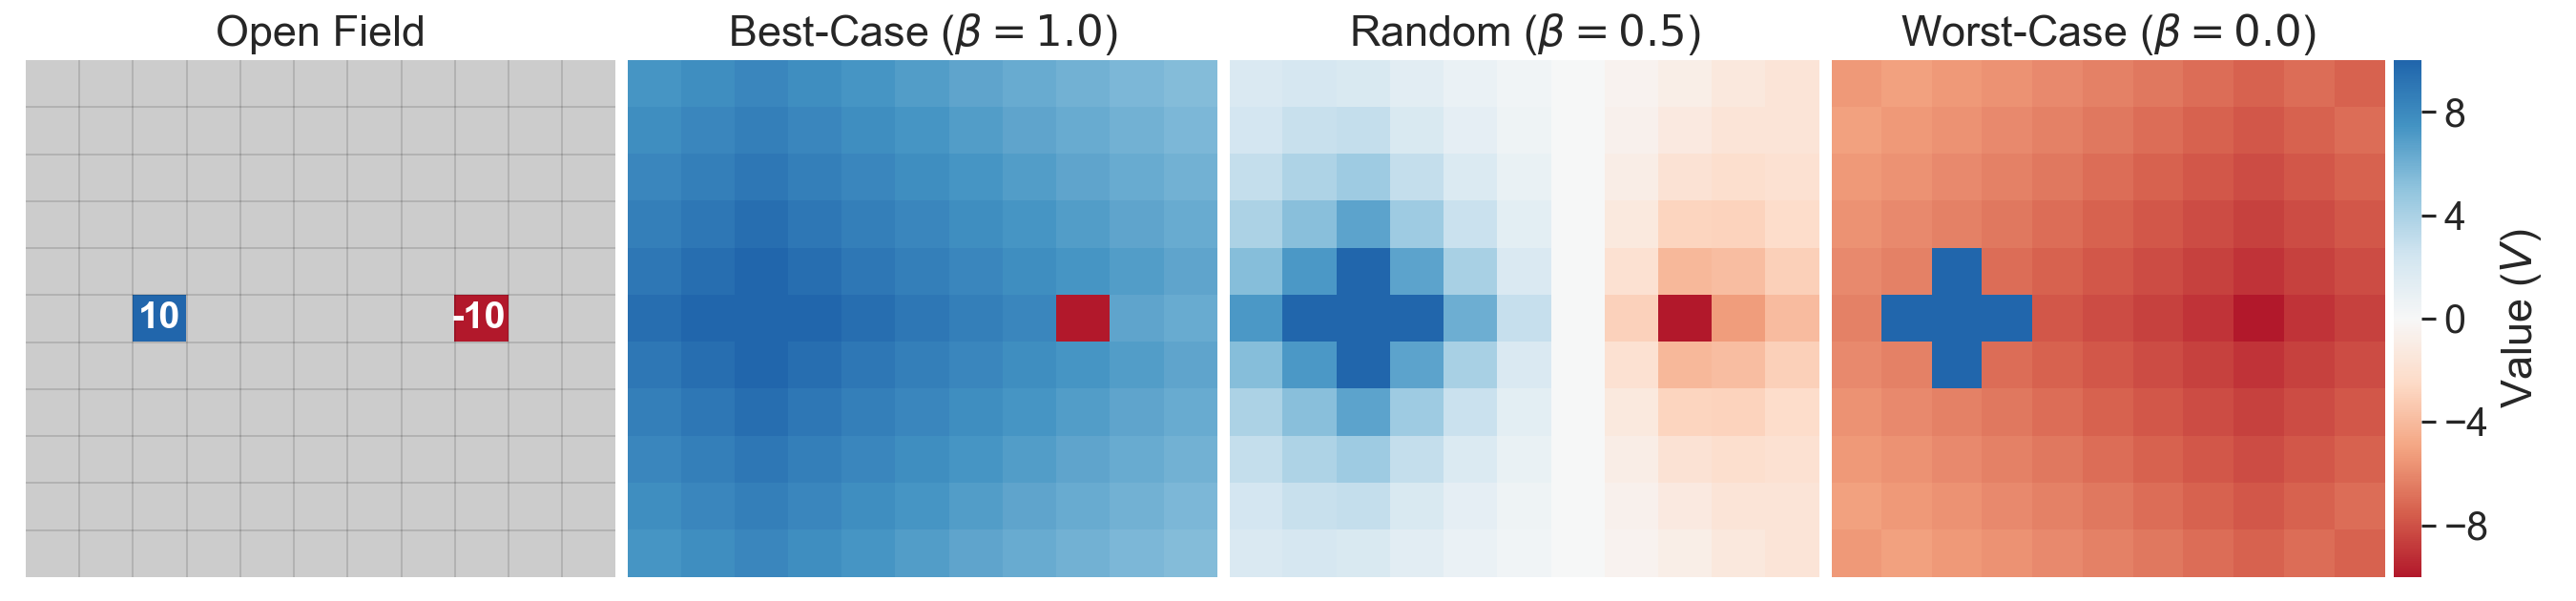
\includegraphics[trim={0 0 0 0},clip]{../figures/01_field.png}}%
  }
  \par \textbf{Figure 1:} The open field is a deterministic gridworld with only one rewarding (blue) and aversive (red) state (A). For an optimistic agent ($w=1$), all states (other than the harmful state) take on positive value (B). For a pessimistic agent ($w=0.5$), negative value spreads from the source to antecedent states (C). With increasing pessimism ($w=0$), the extent of the spread grows worse (D). (Parameters: $\gamma = 0.95$)
\end{figure}

The long-run value estimates learned by an optimistic agent (i.e. an agent expecting to be able to follow a reward-maximizing policy now and in the future) reflect this (Figure 1b). For an optimistic agent, all states in the open field environment, sans the harmful state itself, take on a positive value. This is unsurprising insofar that, except for the harmful state, the agent will always encounter a reward in the long-run no matter its starting position in the field.

The same cannot be said for a pessimistic agent. If an agent doubts its future ability to act in according with the optimal policy, then it cannot rule out that, in the future, it may inadvertently encounter the harmful state. This is more so likely if the agent is already proximal to the harmful state. Under this pessimistic belief, the possibility of future harm is no longer zero, as it is for the optimistic agent, and thus negative value can propagate from the states antecedent to harm, back to their respective antecedents and so on. The extent of this spread will depend on the strength of the pessimistic belief (Figures 1c, 1d). With increasing pessimism, harmful outcomes are assigned greater credence and thus exert greater and wider influence on antecedent states.

In sequential decision environments then, a perceived lack of self-efficacy can result in the propagation of negative value from potential future harms. Such a pessimistic agent may correspondingly report an increased likelihood of threat (i.e. a greater number of threatening states), increased severity of threat (i.e. states with more negative value), and fear of states antecedent to the fear source. As such, pessimistic learning can account for two of the hallmark symptoms of the anxiety disorders.

\subsection{Avoidance}

In addition to pessimistic inference, all anxiety disorders share pathological avoidance as core symptom \citep{dsm5, Krypotos2015, Arnaudova2017}. Avoidance behaviors seek to increase or maintain the temporal, physical and/or mental distance between an individual and a threatening situation. Although avoidance is a natural response to danger, excessive avoidance as is observed in anxiety disorders can be highly disruptive to everyday functioning \citep{Salter2004} and frequently function so as maintain anxiety by preventing extinction \citep{Arnaudova2017}. For example, an individual with social anxiety may avoid attending large social events for fear of public embarrassment only to never learn that such worry is not justified.

Avoidance behaviors in anxiety have been studied using a variety of methods. Perhaps the most classic paradigm is the behavioral avoidance test \citep{bandura1977}, wherein participants complete a number of tasks involving a feared object or situation and the number of tasks completed (or lack thereof) is a measure of avoidance. Computerized avoidance tasks have become increasingly common, and increased distance from virtual threat has been found to correlate with anxiety \citep{Bach2014, Bach2017, Sheynin2014}.

There is a long history of models attempting to explain avoidance learning. The fundamental challenge is explaining how an action can be reinforced in the absence of an outcome. Two-factor theory was the explanation for a long while, but suffered from a number of noteworthy criticisms \citep{Krypotos2015}. Recent work has revitalized two-factor theory and integrated it with reinforcement learning \citep{Moutoussis2008, Maia2010}, and in the process addressing several criticisms of two-factor theory. As has been discussed elsewhere \citep{Moutoussis2017}, such accounts only explain the maintenance of avoidance in short timescales, but do not explain why resistant to change and why they do not go away in general.

\begin{figure}
  \centerline{%
    \resizebox{1.0\textwidth}{!}{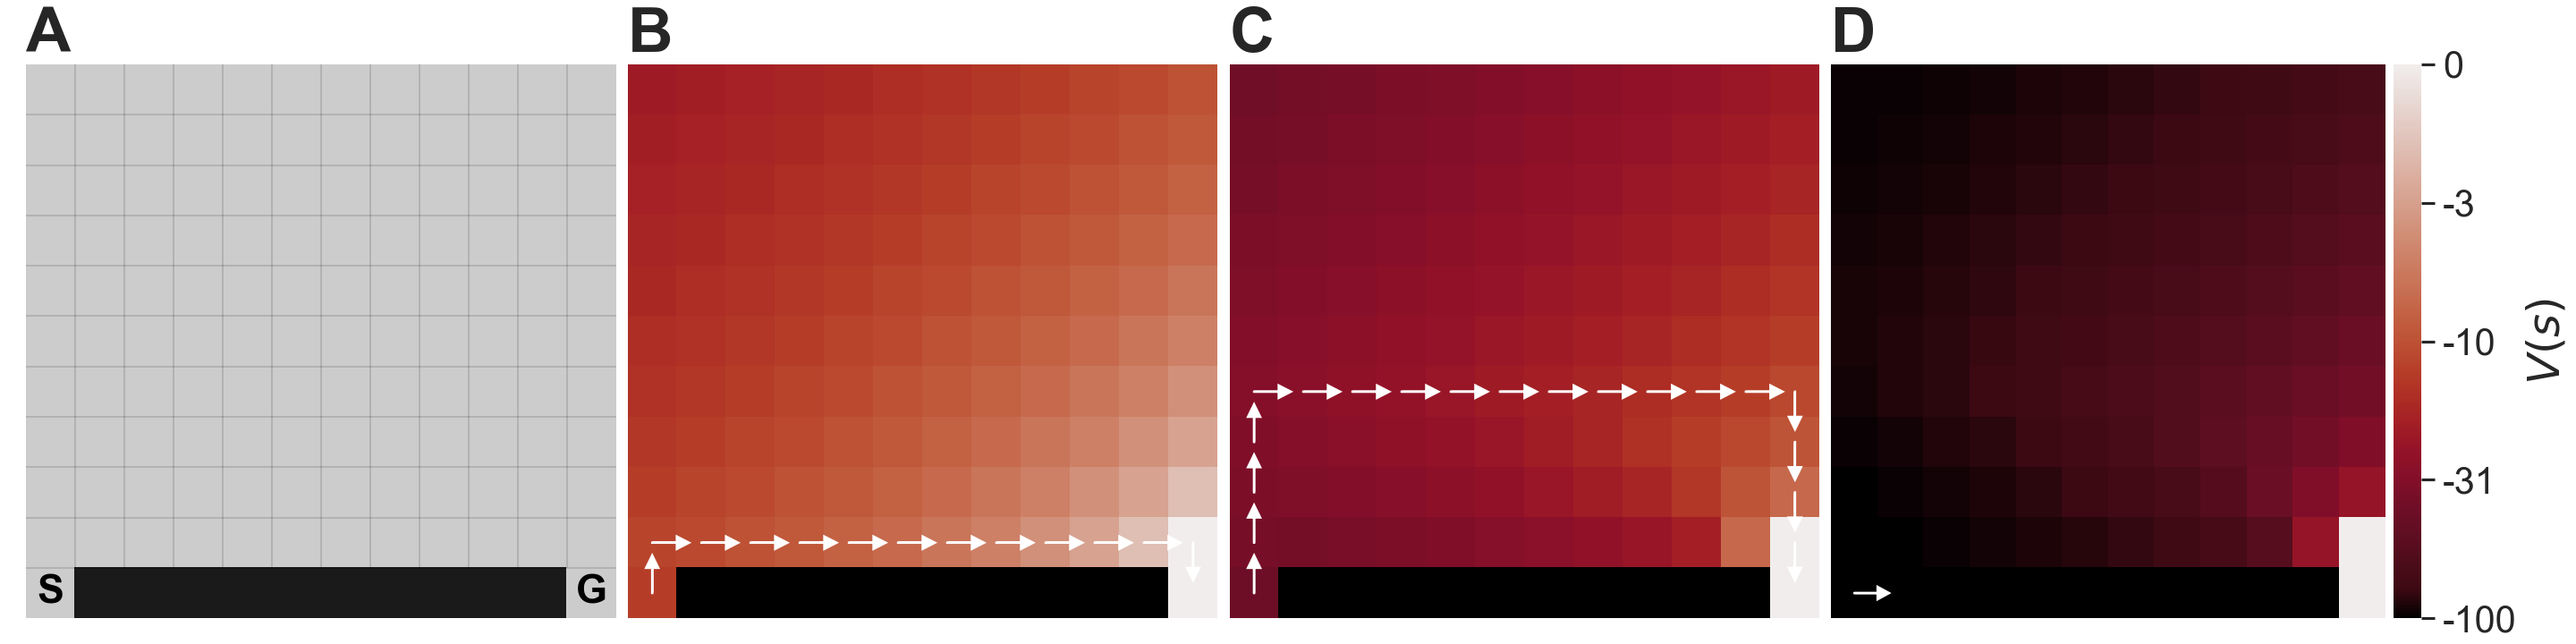
\includegraphics[trim={0 0 0 0},clip]{../figures/02_cliff.png}}%
  }
  \par \textbf{Figure 2:} Cliff-walking is a deterministic gridworld where an agent must navigate from one side (S) to the goal on the other side (G) (A). Every step costs the agent ($r=-1$) but stepping off the cliff results in great harm ($r=-100$). An optimistic agent learns to travel the shortest (loss-minimizing) path along the cliff (B). For a pessimistic agent ($w=0.8$), the potential for harm yields an optimal policy that maintains distance from the cliff's edge (C). With increasing pessimism ($w=0.6$), the agent learns an optimal path off the cliff so as to minimize unnecessary steps prior to its perceived inevitable harm (D). (Parameters: $\gamma = 1$)
\end{figure}

In our second simulation, we demonstrate how pessimistic learning can yield sustained avoidance. In the cliff-walking environment \citep{SuttonBarto1998, SuttonBarto2018, Gaskett2003}, an agent must navigate from a start on side of the map to the other (Figure 2a). The agent experiences a small penalty for every step it takes. The shortest (least costly) path is along the cliff's edge; if the agent steps off the cliff, however, it incurs a much larger penalty. As in the first environment, we assume a deterministic transition structure.

Just as in the first environment, the long-run value estimates by an optimistic agent do not reflect the potential harm of the cliff (Figure 2b). Because this agent (rightfully) expects to act according to the optimal policy in the future (i.e. never step off the cliff), the agent perceives no risk of future disaster and thus the large penalties of stepping off the cliff do not pollute the agent's value estimates. The optimistic agent learns the loss-minimizing policy and walks along the cliff's edge.

This is not the case for the pessimistic agent. As above, when the agent doubts its future ability to act in a reward-maximizing (loss-minimizing) manor, it cannot rule out the possibility of accidentally stepping off the cliff. Thus, the potential for future harm is no longer zero and the large penalties for stepping off the cliff may back-propagate to their antecedent states, and so on. The extent of this spread is dependent on the strength of the pessimistic belief. With increasing pessimism, the optimal policy for the agent is increasingly distance from the cliff's edge (Figure 2c). Surprisingly, at high levels of pessimistic belief, the optimal policy is to immediately step off the cliff (Figure 2d). The reason for this is simple: with high levels of pessimism, the likelihood of disaster grows large enough that any step is simply viewed as adding onto the pain.

Under pessimistic learning then, a perceived lack of self-efficacy can yield the propagation of negative value from potential future harms. In such a scenario, the optimal policy for an agent is to maintain a distance from threat far enough so as to optimally balance the risk of catastrophe with foregone losses. Importantly, these simulations demonstrate the long-run value estimates rather than any momentary value estimates. In other words, the behavioral policy these agents demonstrate will be maintained insofar beliefs about self-efficacy are maintained, irrespective of any momentary noisiness in actual outcomes. Thus, pessimistic learning can account for pathological avoidance in anxiety disorders.

\subsection{Approach-Avoidance Conflict}

Next, we turn our attention to a related phenomenon observed in anxiety: a bias towards avoidance during approach-avoidance conflict \citep{aupperle2010}. In situations where the potential for reward and harm are correlated,
anxiety predicts the tendency to forego reward in favor of minimizing the risk of threat. As a consequence, individuals with anxiety may experience fewer rewards in their environment as compared to non-anxious individuals. For example, an individual with social anxiety may avoid a party for fear of social embarrassment at the expense of positive social interactions with friends. This is a primary mechanism by which clinical anxiety can disrupt everyday functioning.

A relationship between anxiety and biased decision making in approach-avoidance conflict is well-documented in the empirical literature. One common measure is the balloon analog risk task (BART) \citep{Lejuez2002}. The task is straightforward: a participant inflates a virtual balloon, one pump at a time. The more inflated the balloon, the more points the participant earns. With increasing pumps, however, comes the risk of the balloon popping and the loss of all earned points so far. Thus, there is a conflict: a participant can choose to pump the balloon more to earn more points, at the risk of the balloon popping; alternately, the participant can choose to end the trial earlier with fewer points earned. Previous studies have found that anxiety is correlated with earlier leaving times, or a greater tendency to avoid risk \cite{Maner2007, Giorgetta2012}.

\begin{figure}
  \centerline{%
    \resizebox{1.0\textwidth}{!}{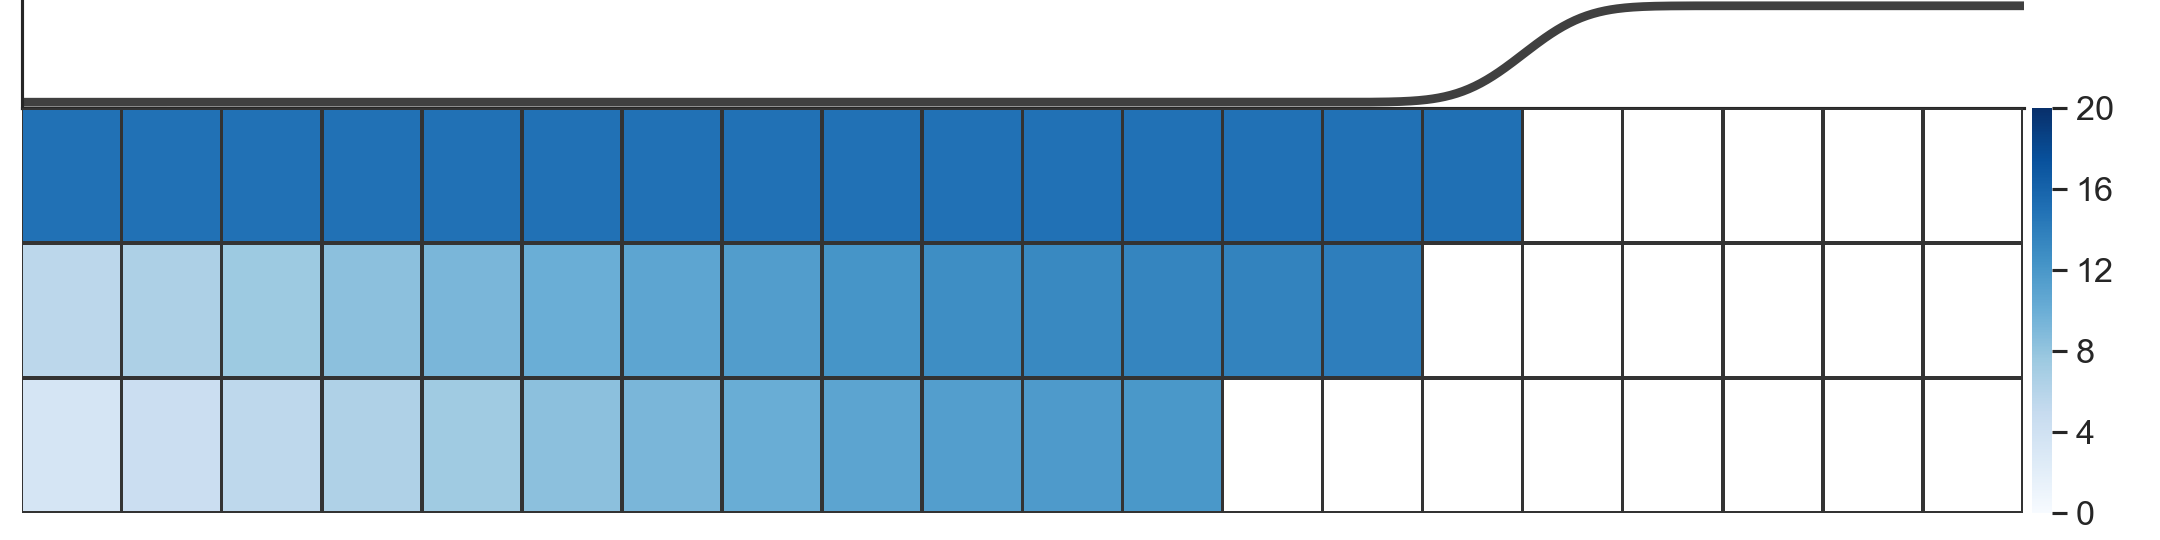
\includegraphics[trim={0 0 0 0},clip]{../figures/03_fid.png}}%
  }
  \par \textbf{Figure 3:} The Balloon Analog Risk Task (BART). Risk of the balloon popping increases with each pump (top row). An optimistic agent ($w=1$) continues to pump until the risk of losing all points earned outweighs the marginal value of one additional pump (second row). A pessimistic agent ($w=0.8$) is less confident that it will make the optimal decision in the future, and thus leaves earlier (third row). Leaving time becomes sooner with increasing pessimism ($w=0.6$) (bottom row). (Parameters: $\gamma = 1$.)
\end{figure}

This result can be accounted for by a loss of confidence in future reliability. A simulation of performance on the BART is shown in Figure 3. For an optimistic agent ($w=1$), the optimal policy is to continue pumping until the risk of popping is all but guaranteed. The optimal policy for pessimistic agents differ. Under a loss of confidence for future action, pessimistic agents cannot be certain they will make optimal choices in the future. As such, negative value propagates backwards resulting in earlier leaving times. The latency of leaving is dependent on the strength of the pessimistic belief.

Interestingly, these results are similar to recent findings regarding flight initiation distance and anxiety \citep{Mobbs2018, Mobbs2019}. Flight initiation distance refers to a measure from behavioral ecology that assesses the leaving time of a foraging animal at risk of predation. In classic flight initiation scenarios, an animal can continue to forage and exploit resources, but the longer it does so the greater the risk it will encounter a predator. Thus, flight initiation scenarios are similar in structure to approach-avoidance conflict and the BART. Recently, \cite{Mobbs2019} found that anxiety is correlated with earlier leaving times in virtual flight initiation tasks. Interestingly, the authors make a distinction between "fast-" and "slow-attacking" predators, and find that trait anxiety is only correlated only in behavioral response to the latter. The findings here draw upon an emerging literature of distinct neural systems mediating "cognitive" vs. "reactive" threat responses, where anxiety evidently impacts the deliberative, cognitive responses. Thus, it is important to note the present theory can account for anxious approach-avoidance behavior in some, but certainly not all, threatening scenarios.

These results may also be related to recent work on the computational mechanisms underlying behavioral inhibition, a temperament linked to anxiety \citep{bach2015, khemka2017}. \cite{bach2015} argues that delayed behavioral responses under threat are normative under the assumption that a pause in behavior (e.g. freezing) can be useful for surveying a threatening environment, avoiding detection by predators, and potentially waiting out a nearby threat. Behavioral inhibition, it is argued, is a useful Pavlovian heuristic that has evolved over time. The current models may predict similar results. Insofar that a loss of confidence in future action yields more negative estimates of action values, then the best action may often be brought closer in value to its alternatives. As such, a pessimistic agent may face increased decision conflict as compared to a non-anxious counterpart and therefore show increased response times. This is not to argue against this particular model of behavioral inhibition, but just to say that our account may yield similar behaviors.

\subsection{Relation to Depression}

As an extension of approach-avoidance conflict, we next want to discuss the relationship between anxiety and depression. Anxiety and depression are highly comorbid, with roughly 45\% of individuals with a lifetime depression diagnosis also diagnosed with at least one anxiety disorder \citep{kessler2015}. Given this, many have clinical theories assume that depression and anxiety are slightly variant manifestations of the same underlying mechanisms involving negative affect (for review, see \cite{jacobson2014}).

Where the two disorders can be distinguished is in relation to rewards and anhedonia; depressive disorders, but not anxiety disorders, are associated with disrupted reward processing. One interesting proposal in the literature is that at least certain types of anhedonic depression are preceded by anxiety \citep{alloy1990, moitra2008, jacobson2014}. Specifically, persistent avoidance has the long-run effect of reducing the likelihood of anxious individuals encountering positive events and activities in their everyday lives. As a consequence, anxious individuals come to expect an absence of reward in their environments and subsequently develop diminished reward motivation and behavioral activation. Recent large-scale epidemiological studies have provided  some empirical support for this claim, finding that anxiety symptoms and behavioral avoidance precede and predict the longitudinal onset of depression (\cite{mathew2011, jacobson2014, kessler2015}; though also see \cite{jacobson2017, plana2019}).

\begin{figure}
  \centerline{%
    \resizebox{1.0\textwidth}{!}{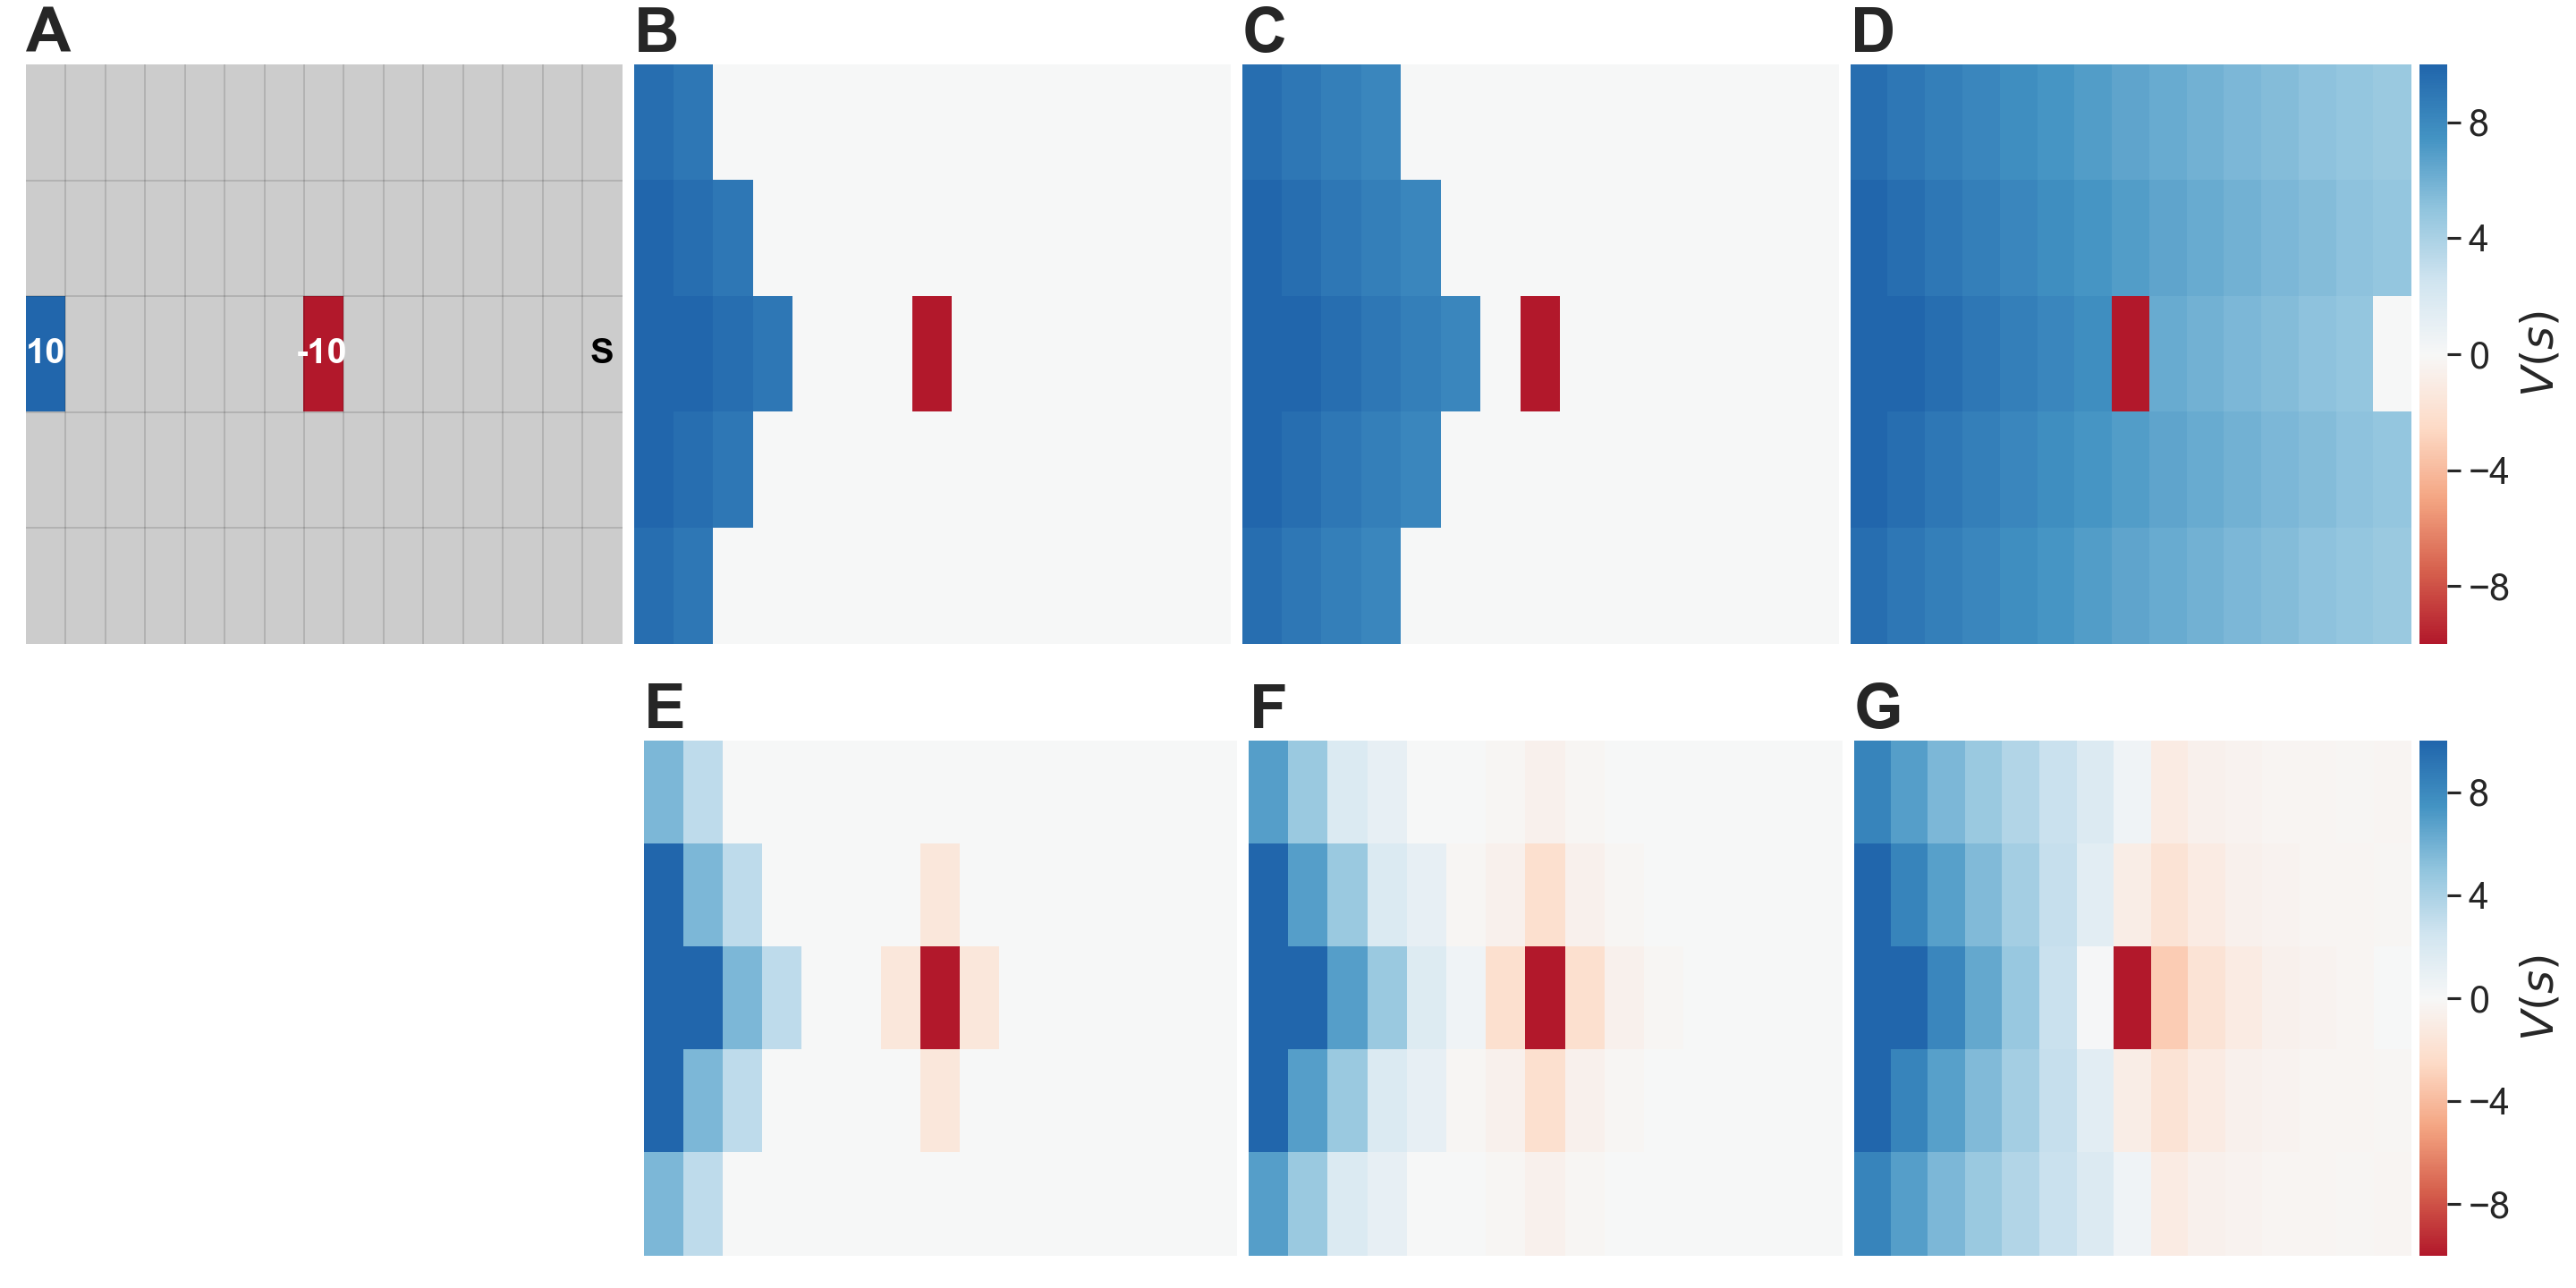
\includegraphics[trim={0 0 0 0},clip]{../figures/06_lh.png}}%
  }
  \par \textbf{Figure 4:} Progression from anxiety to depression. In this open environment, an agent starts opposite a reward (blue) with harm separating them (A). For an optimistic agent ($w=1$), positive value spreads from the reward to the starting tile (Panels B-D, left-to-right). Harm is mitigated through the belief of future self-efficacy. For a pessimistic agent ($w=0.6$), both positive and negative value spread (Panels E-G, left-to-right). Given the agent's closer proximity to harm than reward, the optimal policy for this agent is to stay at the initial state. (Parameters: $\gamma = 0.95$)
\end{figure}

This prediction is easily accommodated by the present model. Simulations of how this might come back is presented in Figure 4. In this environment, there is only one rewarding and harmful state. Just as in the open field environment, the world is deterministic and the harmful state poses no true threat to an agent. An optimistic agent ($w=1$), with a belief in its ability to maintain an optimistic policy, is unfazed by the presence of the harmful state and develops over time an overall positive representation of the value of the environment (Figure 4b-d).

In contrast, a pessimistic agent ($w=0.6$) cannot be certain of its ability to steer clear of future harm. As such, negative value spreads from the harmful state to its antecedent states (Figure 4e-g). Because in this environment risk and reward are correlated (i.e. the agent must approach the harmful state in order to reach the reward given its starting position), the consequence of negatively spreading value is that the optimal policy is to stay in the initial position. Thus, the pessimistic agent adopts a behavioral policy akin to depressive immobility. Moreover, reward is inaccessible to this agent such that its positive expectations of the environment are also diminished. In summary, a loss of confidence in future reliability can result in behavioral policies that resemble depressive-like states in environments with correlated risk and reward.

\subsection{Planning}

In this next section, we review the literature on aversive pruning. In large, multi-step sequential decision environments, the space of all possible sequences of choices grows exponentially larger with increasing sequence length. As such, it is infeasible for decision making agents to exhaustively explore all possible sequences select that which maximizes reward from the entire set. Heuristics for narrowing the search space then are not only plausible but beneficial for a decision making agent.

One such heuristic that has been proposed in the literature is aversive pruning \citep{Huys2012}. Aversive pruning is defined as a Pavlovian response to encountering a large loss in planning such that sequences involving large losses are discarded from further evaluation. An example of such a scenario is presented in Figure 5. The prediction in this decision tree environment is that an agent would discard the branch of the decision tree involving an immediate large negative loss, even though this branch objectively contains the reward maximizing (loss minimizing) sequence of choices.

\cite{Huys2012} (and later \cite{Lally2017}) tested this prediction in this particular choice environment. Participants received extensive training in this decision tree environment (first without outcomes and then later with rewards) in order to facilitate planning. In free-planning trials, many participants exhibited this Pavlovian bias, rejecting choice sequences which involved the large loss even when the sequence was objectively reward maximizing (loss minimizing). Importantly \cite{Huys2012} and \cite{Lally2017} found the degree of aversive pruning was correlated with depressive and anxiety symptoms, respectively.

\begin{figure}
  \centerline{%
    \resizebox{1.0\textwidth}{!}{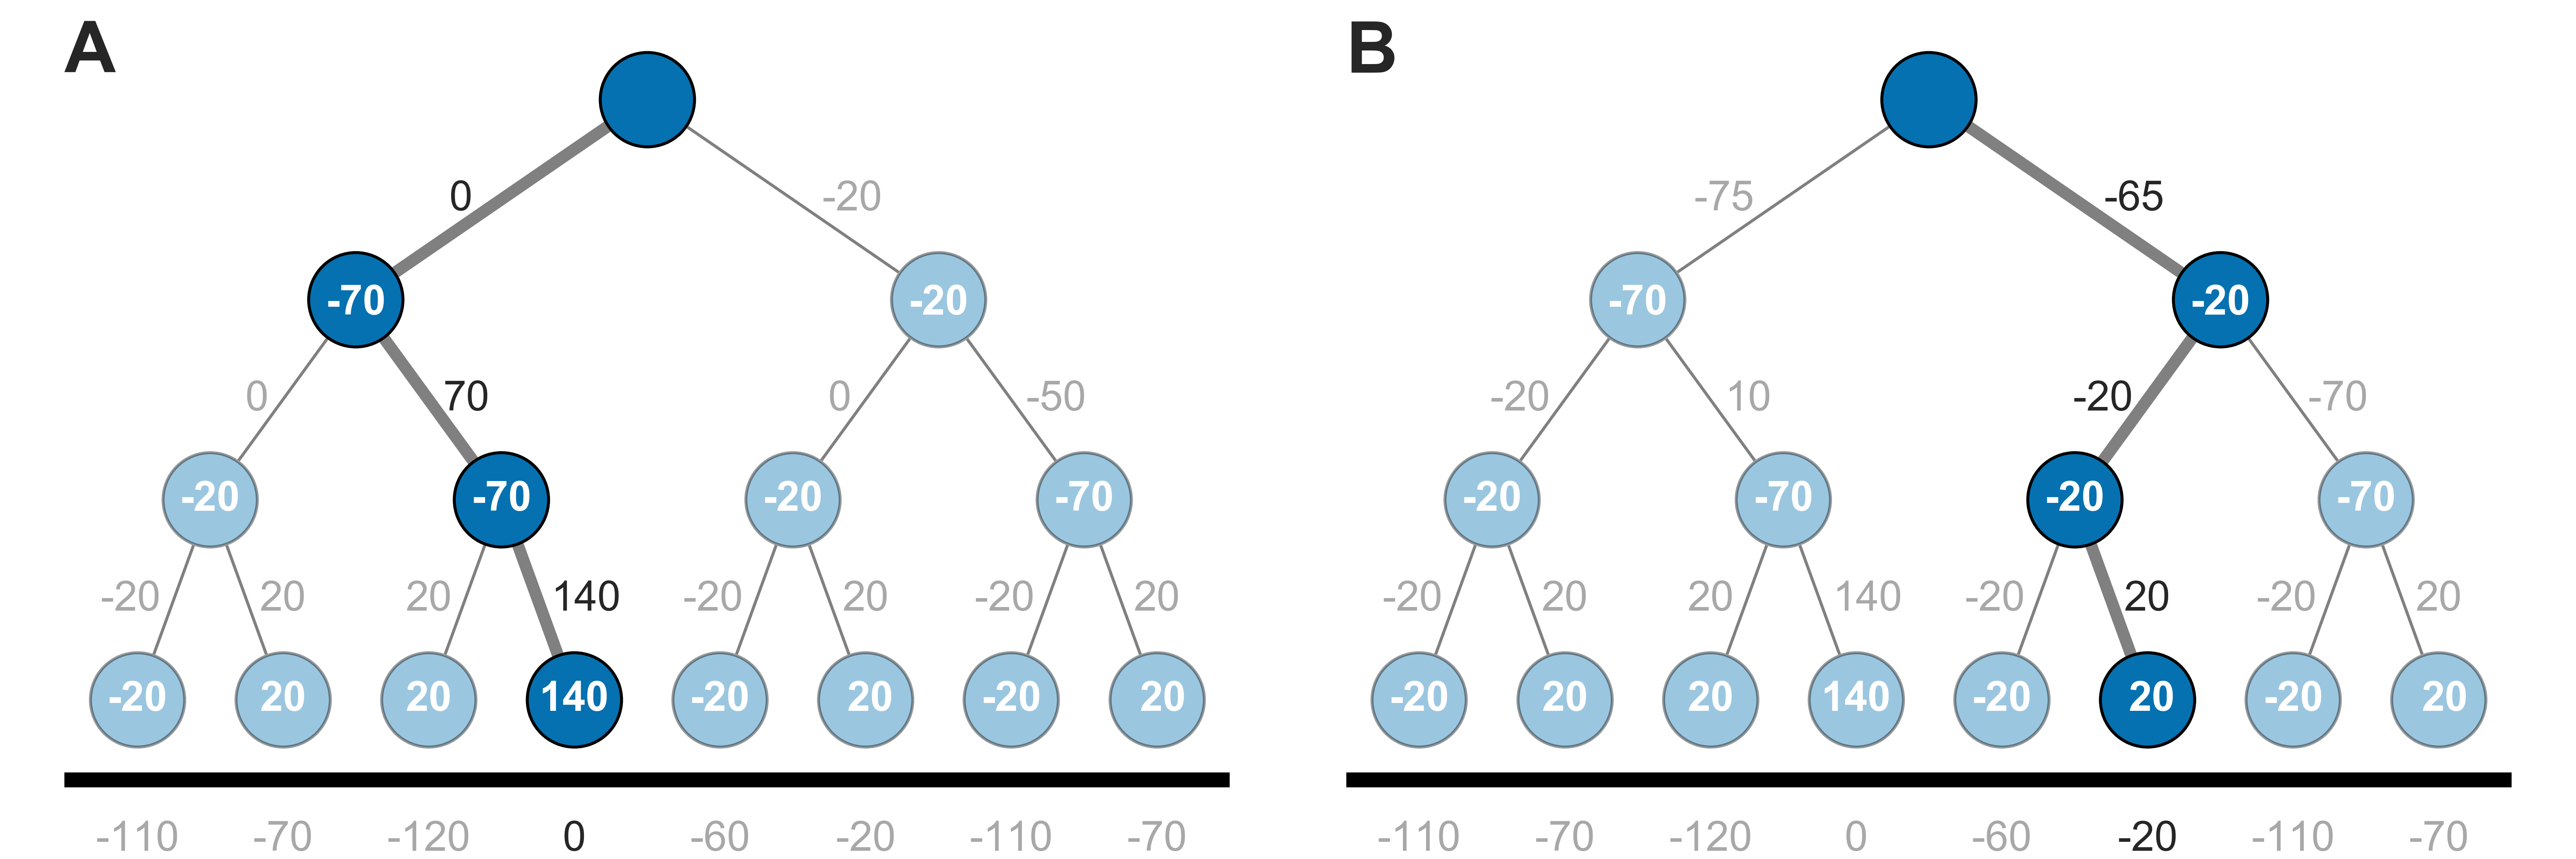
\includegraphics[trim={0 0 0 0},clip]{../figures/04_tree.png}}%
  }
  \par \textbf{Figure 5:} The decision tree environment from \cite{Huys2012} and \cite{Lally2017} (A). An optimistic agent ($w=1$) learns the optimal loss-minimizing policy through the initial large loss (B). A moderately pessimistic agent ($w=0.75$) will find both arms equally preferable insofar that it is less confident it will be able to execute optimal future choices (C). More pessimistic agents comes to prefer the branch without the large loss so as to avoid being unable to recoup the large initial loss (D).
\end{figure}

The aversive pruning principle makes tremendous sense and draws on a robust literature of heuristics and computational shortcuts for circumventing computationally intractable cognitive processes. It is important to note, however, that a control interpretation also makes similar predictions. Figure 5b-d shows the preferred routes of simulated agents in the same environments under increasingly pessimistic expectations of future actions. As can be observed, pessimistic agents are similarly likely to avoid the branch with the large loss, though for different reasons. Under the pessimistic case, the agent is increasingly less confident that the large gains later in sequence will be realized; as such, the agent is less confident that the initial large loss will be offset. Consequently, pessimistic agents would prefer the branch with smaller losses (even if this is objectively suboptimal). This prediction is similarly consistent with the finding that avoidance of the initial large loss is correlated with anxiety \cite{Lally2017}.

%% An interpretation like this would be consistent with reduced beliefs in one's own competency in such an environment. This is not strictly surprising. Planning multi-choice sequences even in relatively simple environments like those used in these experiments still ostensibly require working memory ability to keep in mind the possible consequences along each branch. Insofar that working memory ability is disrupted in anxiety disorders \citep{Moran2016}, a pessimistic belief may be justified and possibly optimal.

It is worth noting that these two alternate accounts can be disentangled through slight manipulations of the choice environment presented above. Aversive pruning and loss of confidence make similar predictions when a large loss begins a sequence, but not necessarily when a large potential loss comes later in a sequence. In the loss of confidence view, the potential for large loss late in a sequence negatively impacts the estimated value of actions early in the sequence; this is not true for aversive pruning. Identifying such choice sequences in the decision tree task may help identify whether this sort of inference is present in individuals with anxiety performing the task.

\subsection{Free Choice Premium}

In this final section, we propose based on the present theory that anxiety should be inversely related to the free choice bias. If an agent is confident in their future decision making abilities, then it follows that situations in which an individual is able to make a future choice should be preferable to situations in which an individual is not. At worst, an agent is no better off than if they had not made a choice; at best, an agent is better able to steer themselves toward desirable outcomes. Such is the logic that underlies an emerging literature suggesting that choice is inherently valuable \citep{Leotti2010}.

This free choice premium has been observed across several behavioral experiments \citep{Suzuki1997, Leotti2011, Leotti2014, Cockburn2014} using a variety of decision paradigms. For the present purposes, we will describe the experiments presented in \citep{Leotti2011, Leotti2014}. In these experiments, participants complete a two-stage decision making task (Figure 6). In the first stage, participants are make a choice between two cues: one leading to free choice and the other leading to a fixed choice. In the second stage, participants are able to choose between a second set of cues (free choice) or are forced to choose a cue (fixed choice). Unbeknownst to participants, all cues yield reward following the same outcome distribution; thus, no cue is advantageous in the long-run. The free choice premium is measured as a preference for the cue leading to free choice. \cite{Leotti2011, Leotti2014} find participants still prefer the free choice cue, despite this conferring no objective benefit to participants.

Insofar that the free choice premimum is contingent on an agent's belief in its future ability, it stands to reason that this free choice premium should be absent in individuals with anxiety and a loss of confidence. Simulations of this effect are presented in Figure 6. Simulated agents complete an experiment similar to that used in \cite{Leotti2011, Leotti2014}. In contrast to optimistic agents, the value of the worst action in the free choice arm back-propagated to the free-choice cue in pessimistic agents. With increasing pessimism then, the free choice option is less preferable than the fixed choice arm. As a result, pessimistic learners, on average, do not exhibit a bias towards the free choice arm. To our knowledge this prediction has not been empirically tested.

\begin{figure}
  \centerline{%
    \resizebox{1.0\textwidth}{!}{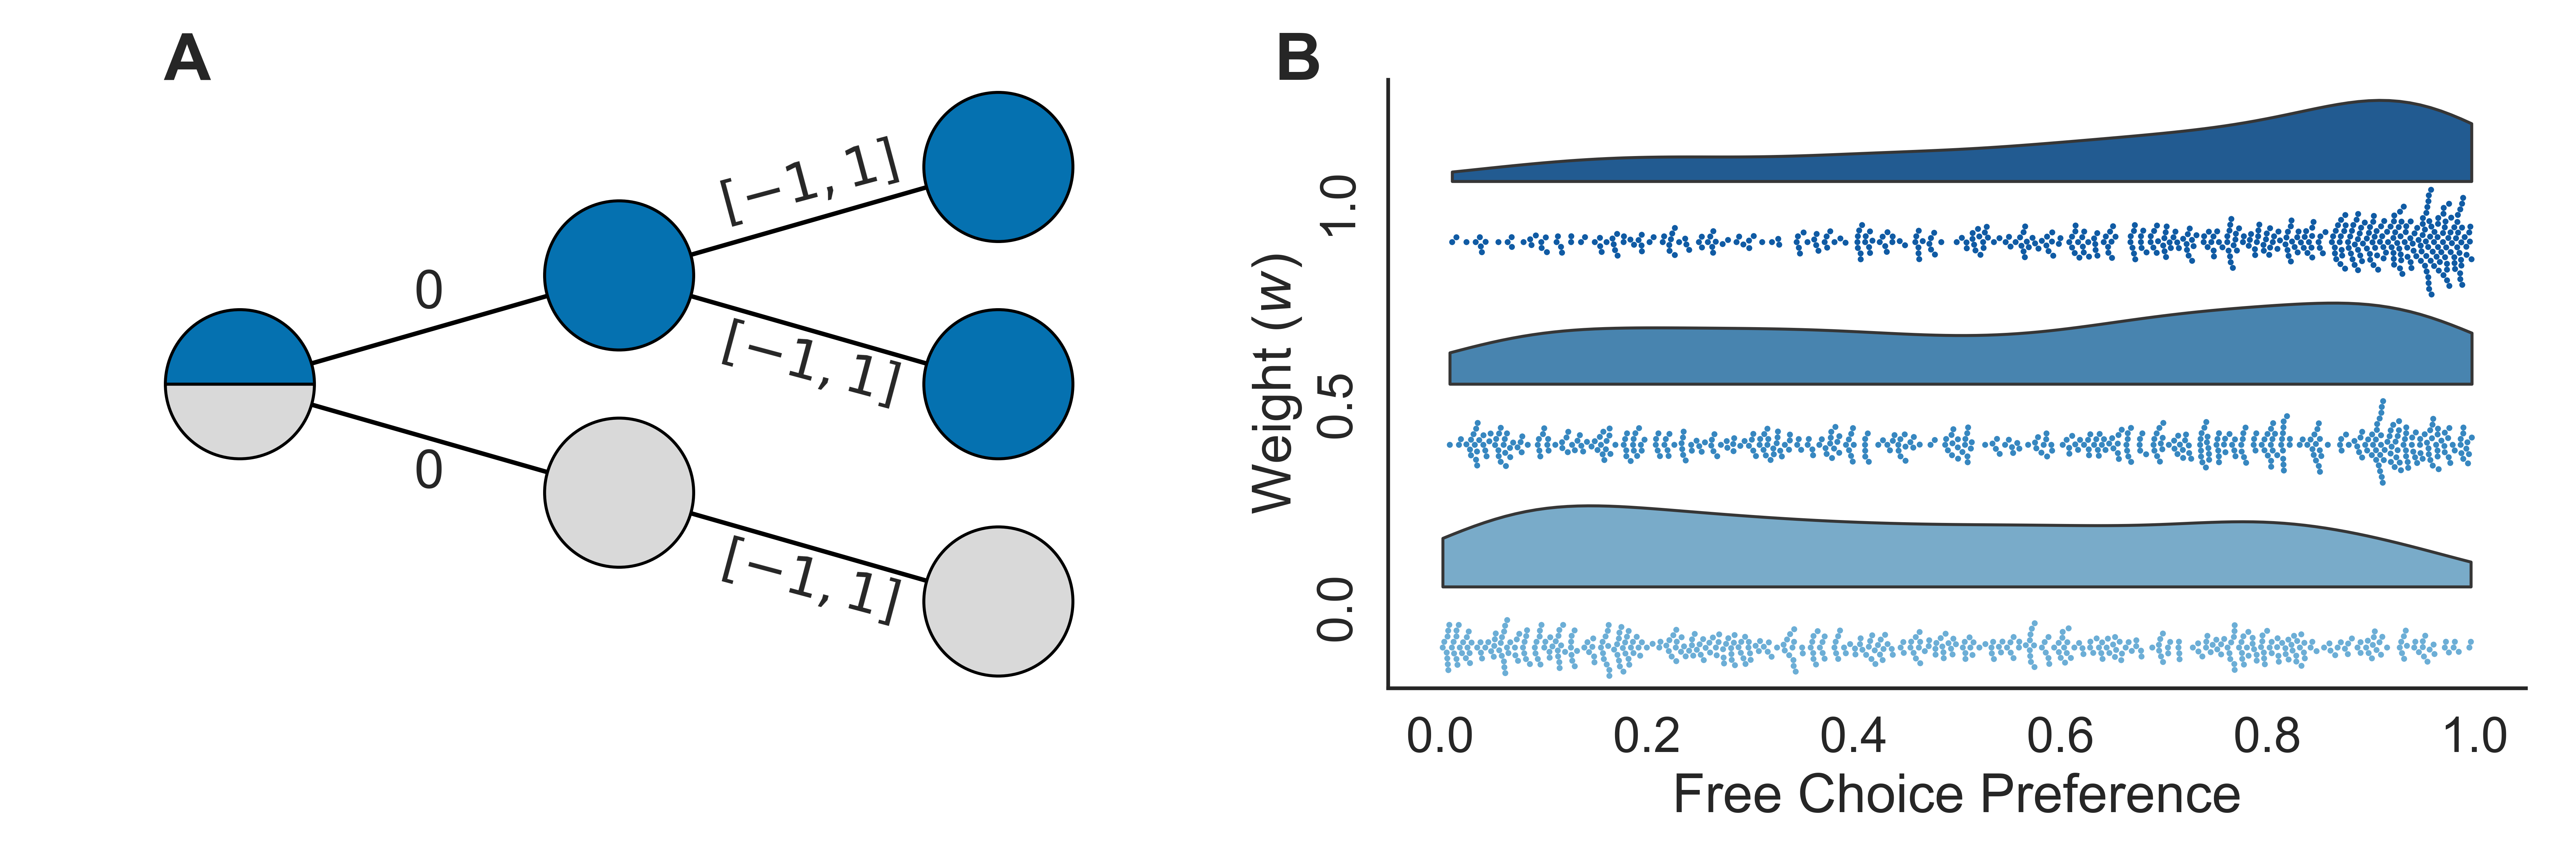
\includegraphics[trim={0 0 0 0},clip]{../figures/05_choice.png}}%
  }
  \par \textbf{Figure 6:} Schematic of the free choice bias tasks used in \cite{Leotti2011, Leotti2014} (A). The free choice bias is diminished in increasingly pessimistic agents (B).
\end{figure}

\section{Discussion}

Central to the acquisition and maintenance of anxiety disorders are symptoms including pessimistic inference, second-order conditioning, and persistent avoidance. In this article, we presented a simple computational account of these aberrations in learning and decision making. Specifically, we showed how a loss of confidence in the reliability of the future self and/or the environment can effectively backpropagate negative value across states of the environment. The result of this process are a series of inferences and behaviors resembling those observed in clinical anxiety. Though this is by no means a complete account of anxiety, the present model helps to explain the core symptoms of anxiety under one unifying framework.

Importantly, this computational account draws upon a longstanding recognition of the importance of perceived control to the development and maintenance of anxiety disorders. Central to many prominent theories of anxiety in the clinical literature highlight is a perceived lack of control. For example, learned helplessness theory and its successors claim that pathological anxiety results from a stable belief that the environment is uncontrollable, such that threat cannot be effectively mitigated. In contrast, Bandura's self-efficacy theory of anxiety posited that a lack of confidence in one's own ability to effectively handle threat was central to the pathogenesis of anxiety. Later theories, such as the triple vulnerability model, are equivocal as to whether an unreliable future environment or self is the root cause of anxiety, but highlights control beliefs as being a necessary compontent for developing anxiety. As we note above, the present model can accommodate either effect. Insofar that the state transition function and future state-action function are multiplicative, a pessimistic change to either should make similar predictions. It is possible that under certain conditions they may predict different outcomes. Future work may tease these apart, as they may be interesting for guiding treatment.

It is worth noting that we are not the first to attempt to formalize a theory of control in MDP. \cite{HuysDayan2009} provided a first computational account of learned helplessness through simple models of action-outcome contingencies. \cite{HuysDayan2009} found that training an agent first in an unreliable environment led to later impaired learning, akin to early learned helplessness experiments, by virtue of the prior of controllability. This provides a nice demonstration of learning impairment of action-outcome contingencies. Importantly, our accounts differ in at least three respects. First, we consider sequential decision environments, which is necessary for more accurately characterizing the symptoms of anxiety disorders. Second, our account specifies a mechanism by which the worst outcomes are realized; in their account, the world simply becomes random. This pessimism seems closer to what is observed in anxiety disorders. Finally, our account accounts for the persistence of these symptoms. Presumably, their model would eventually learn to escape with additional training; our account shows aberrant behaviors in the optimal (long-run) policy.

In this article, we discussed two mechanisms by which negative values can spread, through the state transition distribution and future state-action action. There is a third that we did not address here: that of the state itself. Here we assumed that states were fully observable; in other words, there was no uncertainty about the state an agent was currently occupying. In partially-observable Markov decision problems, the state itself must be inferred from external and internal variables. This is yet another means by which bad value can spread if undue likelihood is granted to undesirable or aversive states. This ideas has previously been proposed to explain some symptoms in anxiety \citep{Paulus2012}, and not without good reason. Anxiety disorders involve negatively biased interpretation of ambiguous percepts \citep{Hartley2012}, which may result in aberrant planning and increased avoidance for similar reasons to those described above. This is an area for future research.

In this article, we have explored a computational principle of approach and avoidance learning in sequential decision environments. We have not discussed, however, the particular psychological or neurobiological mechanisms by which this sort of learning may take place. This issue has been discussed in detail elsewhere \citep{Bishop2018}, but we briefly discuss a few possibilities here. One possibility is in biased sampling. If decision making and planning may rely on internal sampling from previously experienced episodes in order to make predictions about future value, then biased sampling may result in maladaptive decision making. Recent work has shown how finite sampling during planning can result in risk aversion and the overrepresentation of low probability but strongly negative outcomes (Lieder et al., 2018). Such a mechanism is prima facie in line with results showing the availability in memory of negative outcomes being higher for patients with anxiety \citep{Borkovec1999, Miranda2007}. Another possibility are an overreliance on Pavlovian heuristics, such as aversive pruning \citep{Huys2012,Lally2017}. As discussed above, future work should tease apart the predictions of our model and the aversive pruning heuristic.

Several recent studies have found evidence suggesting increased learning rates for negative reward prediction errors in individuals with elevated levels of anxiety \citep{Harle2017, Garrett2018, Aylward2019}. Though incearned learning from negative reward prediction errors may result in anxiety-like behaviors, these are likely not the sole cause of anxiety disorders for the reasons discussed above. Future research might investigate the relationship of prior beliefs about the reward statistics of the environment and learning to positive and negative prediction errors. A separate interestisng possibility is prioritized replay (Russek et al., 2017; Mattar and Daw, 2018). Offline replay of previous experiences (through hippocampal mechanisms) are known to facilitate learning. It has been proposed that biased replay could bias value estimates (Gagne et al., 2018).

\bibliographystyle{vancouver-authoryear}
\bibliography{citations}

\section{Appendix}

\begin{algorithm}
  \caption{Value Iteration}

  \State Algorithm parameter: a small threshold $\theta > 0$ determining accuracy of estimation
  \State Initialize $V(s)$, for all $s \in S$ arbitrarily, except that $V(terminal) = 0$
  \State
  \While{$\Delta > \theta$}
    \State $\Delta \leftarrow 0$
    \Loop \ for each $s \in S$
      \State $v \leftarrow V(s)$
      \State $ V(s) = \max_a \sum_{s',r} p(s',r|s,a) \left[ r + \gamma V(s') \right] $
      \State $\Delta \leftarrow \max(\Delta, |v - V(s)|)$
    \EndLoop
  \EndWhile

\end{algorithm}

\end{document}
